\section{Auswertung}

Vorgehen bei der Erstellung der Graphik\\[5ex]

\begin{figure}[ht]
	\centering	
	\begin{minipage}{1\textwidth}
	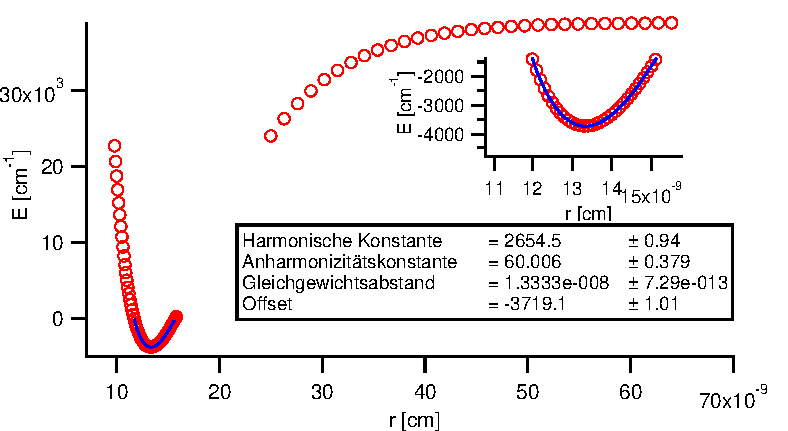
\includegraphics[width=\columnwidth]{Bilder/HCLGraph.pdf}
	\end{minipage}
	
	
	\caption{mit IgorPro gemacht. HCL über morsefit}
	
	
	%\label{HCLplot}
\end{figure}

\begin{figure}[ht]
	\centering	
	\begin{minipage}{1\textwidth}
	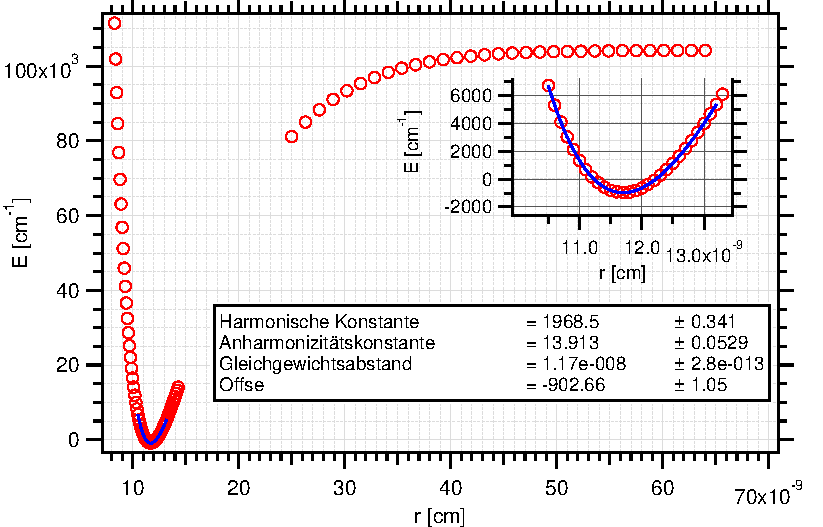
\includegraphics[width=\columnwidth]{Bilder/Graph2.pdf}
	\end{minipage}
	
	
	\caption{mit IgorPro gemacht. CO über morsefit}
	
	
	%\label{COplot}
\end{figure}


\begin{equation} 
	\label{eq:de}
		D_e \approx \frac{\tilde{\nu}_e^2}{4 \tilde{\nu}_e x_e}
\end{equation}

\begin{equation} 
	\label{eq:de}
		D_e \approx \frac{2654.5^2}{4\cdot60.006} ~\si
{cm^{-1}}  \approx  \SI[mode=math]{29356.94}{cm^{-1}} 
\end{equation}

\begin{itemize}
 \item \FPeval{\result}{clip((2654.5^2)/(60.006*4))}%
    $\result$
\end{itemize} 
\section{Fehlerrechnung und Konstante B}
Die Rotationskonstante $B$, sowie der Fehler $\Delta B$ berechnen sich gemäß den Gleichungen :::.
\begin{align}
\label{eq:B}
B 	
   			&= \frac{\hbar}{4 \cdot \pi \cdot c \cdot \mu  \cdot r_e^{2}}
   			\\
   			&= konst.\cdot\frac{1}{\mu  \cdot r_e^{2}}
   			\\
\Delta B	
   			&=  \left|\frac{\delta B}{\delta r_e}\right|\cdot\Delta r_e =konst. \cdot\left|\frac{-2}{\mu \cdot r_e^{3}  }\right|\cdot \Delta r_e   			 
\end{align}
Dabei werden zur Vereinfachung die Naturkonstante in einer Konstante $konst.$ in Gleichung ::: zusammengefasst.


\begin{align}
\label{eq:konst}
konst.&= 			 \frac{\SI[mode=math]{1.054571800e-34}{kg.m.s^{-1}}}{4\cdot 3.14159265359 \cdot \SI[mode=math]{299792458}{m.s^{-1}}}=\SI[mode=math]{2.799274682e-44}{kg.m}  				
\end{align}

\subsection*{HCl}
Für HCl ergibt sich somit, unter Verwendung der durch den Fit ausgegeben Gleichgewichtsabstand $r_e$ und dem dazugehörigen absoluten Fehler $\Delta r_e$
\begin{align}
\label{eq:re_HCL}
r_e &= 1.3333 \cdot 10^{-8} ~\si{cm}=\SI[mode=math]{1.3333e-10}{m}
\\
\Delta r_e &= 7.29 \cdot 10^{-13} ~\si{cm}=\SI[mode=math]{7.29e-13}{m}
\end{align}
,sowie der in Gleichung \ref{eq:mu_HCL} berechneten reduzierten Masse $\mu$
\begin{align}
\mu&= \frac{m(H)\cdot m(Cl)}{m(H)+m(Cl)}\notag\\
\mu&= \frac{1\cdot35}{1+35} ~\si{u}=\frac{35}{36}~\si{u}=\SI[mode=math]{1.614412705e-27}{kg}\label{eq:mu_HCL}
\end{align}
die in Gleichung \ref{eq:B_HCL} berechnete Rotationskonstante $B$
\begin{align}
\label{eq:B_HCL}
B &=\frac{\SI[mode=math]{2.799274682e-44}{kg.m}}{\SI[mode=math]{1.614412705e-27}{kg}\cdot\SI[mode=math]{1.3333e-20}{m^{2}}}
&=\SI[mode=math]{}{m^{-1}}
=\SI[mode=math]{}{cm^{-1}}
\end{align}


,sowie der absolute Fehler$\Delta B$  gemäß Gleichung  \ref{eq:DeltaB_HCL}.  
\begin{align}
\Delta B &= \left|-2\cdot \frac{\SI[mode=math]{2.799274682e-44}{kg.m}}{\SI[mode=math]{1.614412705e-27}{kg}\cdot\SI[mode=math]{1.3333e-30}{m^{3}}}\right| \cdot \SI[mode=math]{7.29e-15}{m}
\notag\\
&= \label{eq:DeltaB_HCL}
\end{align} 


\subsection*{CO}
Für CO ergibt sich somit, unter Verwendung der durch den Fit ausgegeben Gleichgewichtsabstand $r_e$ und dem dazugehörigen absoluten Fehler $\Delta r_e$
\begin{align}
\label{eq:r_CO}
r_e &= 1.17 \cdot 10^{-8} ~\si{cm}=\SI[mode=math]{1.17e-10}{m}
\\
\Delta r_e &= 2.8 \cdot 10^{-13} ~\si{cm}=\SI[mode=math]{2.8e-15}{m}
\end{align}
 sowie der in Gleichung \ref{eq:mu_CO} berechneten reduzierten Masse $\mu$
\begin{align}
\mu&= \frac{m(H)\cdot m(Cl)}{m(H)+m(Cl)}\notag\\
\mu&= \frac{12\cdot16}{12+16} ~\si{u}=\frac{48}{7}~\si{u}=\SI[mode=math]{1.138655165e-26}{kg}\label{eq:mu_CO}
\end{align}
die in Gleichung \ref{eq:B_CO} berechnete Rotationskonstante $B$
\begin{align}
\label{eq:B_CO}
B &=\frac{\SI[mode=math]{2.799274682e-44}{kg.m}}{\SI[mode=math]{1.13655165e-26}{kg}\cdot\SI[mode=math]{1.17e-20}{m^{2}}}
&=\SI[mode=math]{210.50}{m^{-1}}
=\SI[mode=math]{2.10}{cm^{-1}}
\end{align}


,sowie der absolute Fehler$\Delta B$ gemäß der  Gleichung \ref{eq:DeltaB_CO}.  
\begin{align}
\Delta B &= \left|-2\cdot \frac{\SI[mode=math]{2.799274682e-44}{kg.m}}{\SI[mode=math]{1.13655165e-26}{kg}\cdot\SI[mode=math]{1.17e-30}{m^{3}}}\right| \cdot \SI[mode=math]{2.8e-15}{m}
\notag\\
&=0.01178849883\label{eq:DeltaB_CO}
\end{align} 









 %ab hier die Fehlerrechnung  
 
%&eingesetzt in die Gleichung \ref{eq:de} ergibt sich somit:
%hier eine Abblidung\\[5ex]
%Anpassung der Parameter an die Morsefunktion\\[5ex]
%Rechnerische Bestimmung der molekularen Konstanten 
%aus der Morsefunktoin\\[5ex]
%Tabelarische Auflistung für CO und HCl + Literaturdaten\\[5ex]
%Prognose des Rotationsschwingungsspektrum von HF und HCl.

\section{Roationsschwingungsspektrum von HCL und CO bei verschiedenen T}

\begin{figure}[ht]
	
	\begin{minipage}{0.5\textwidth}
	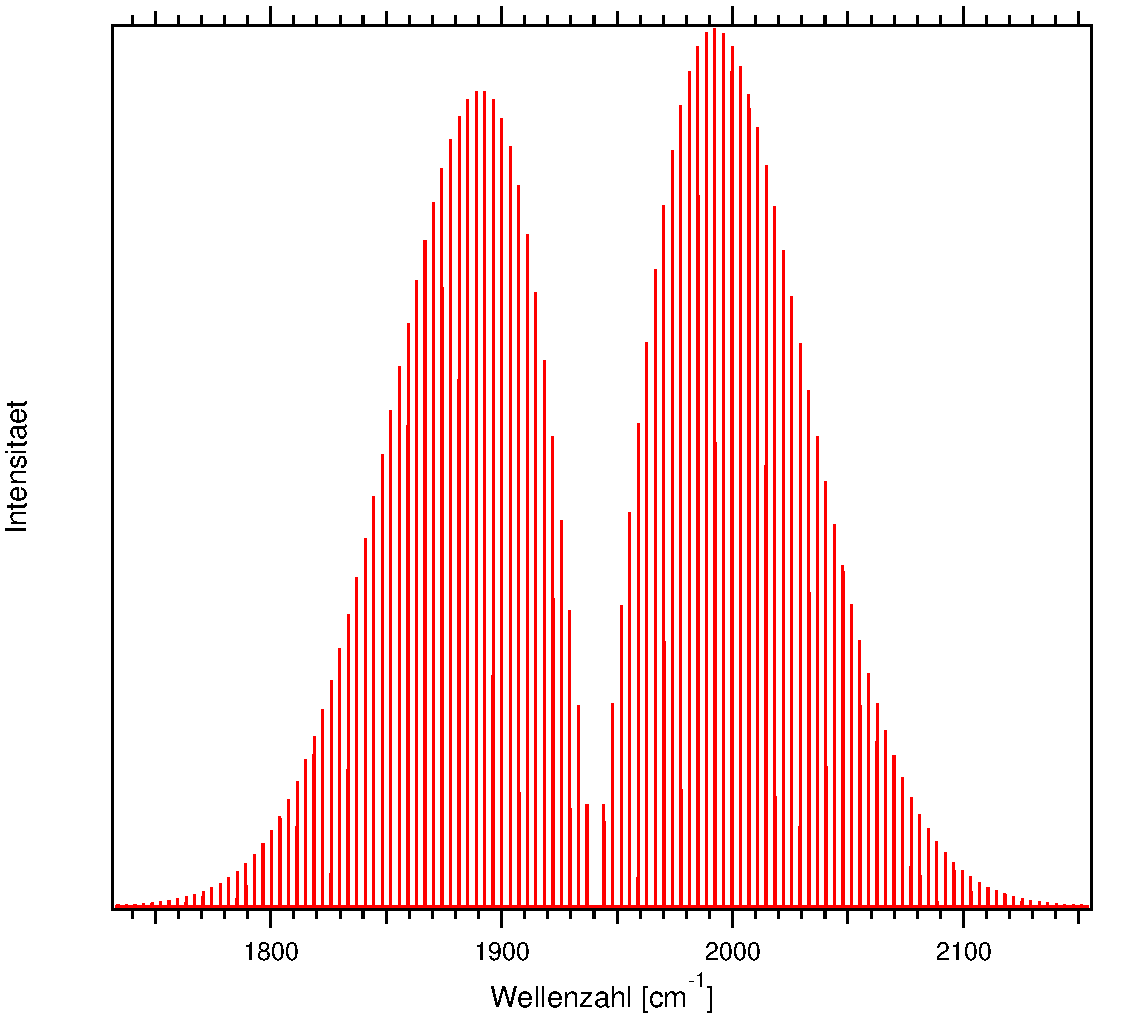
\includegraphics[width=\textwidth]{Bilder/1000CO.pdf}
	\caption{berechnetes Rotationsschwingungsspektrum bei 1000 Kelvin}
	\end{minipage}
\begin{minipage}{0.5\textwidth}
	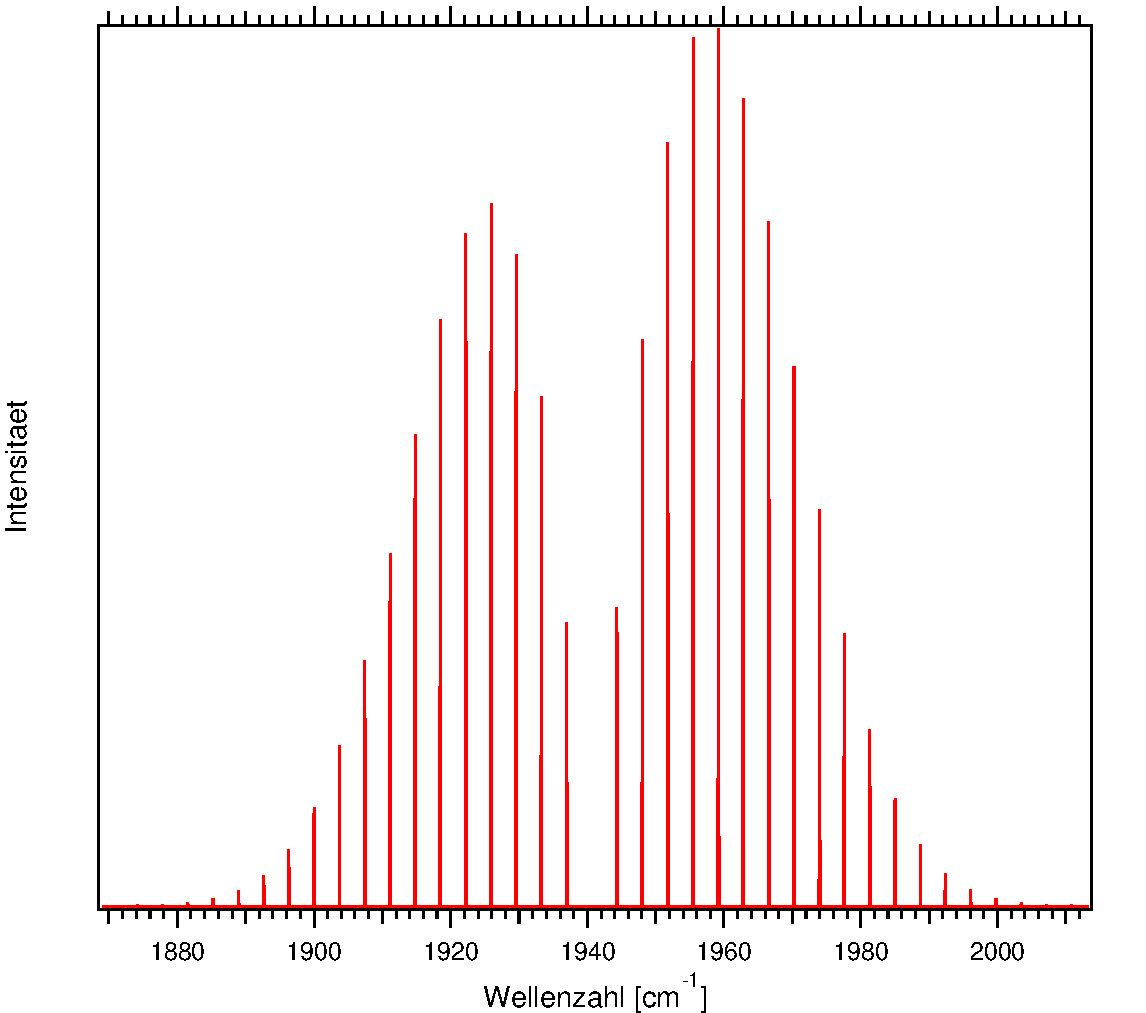
\includegraphics[width=\textwidth]{Bilder/100CO.pdf}
	\caption{berechnetes Rotationsschwingungsspektrum bei 100 Kelvin}
	\end{minipage}	
	
	\caption{CO 1000 und 100 Kelvin}
	
	
%	\label{•}
\end{figure}

\begin{figure}[H]
\centering	
	\begin{minipage}{0.47\linewidth}
	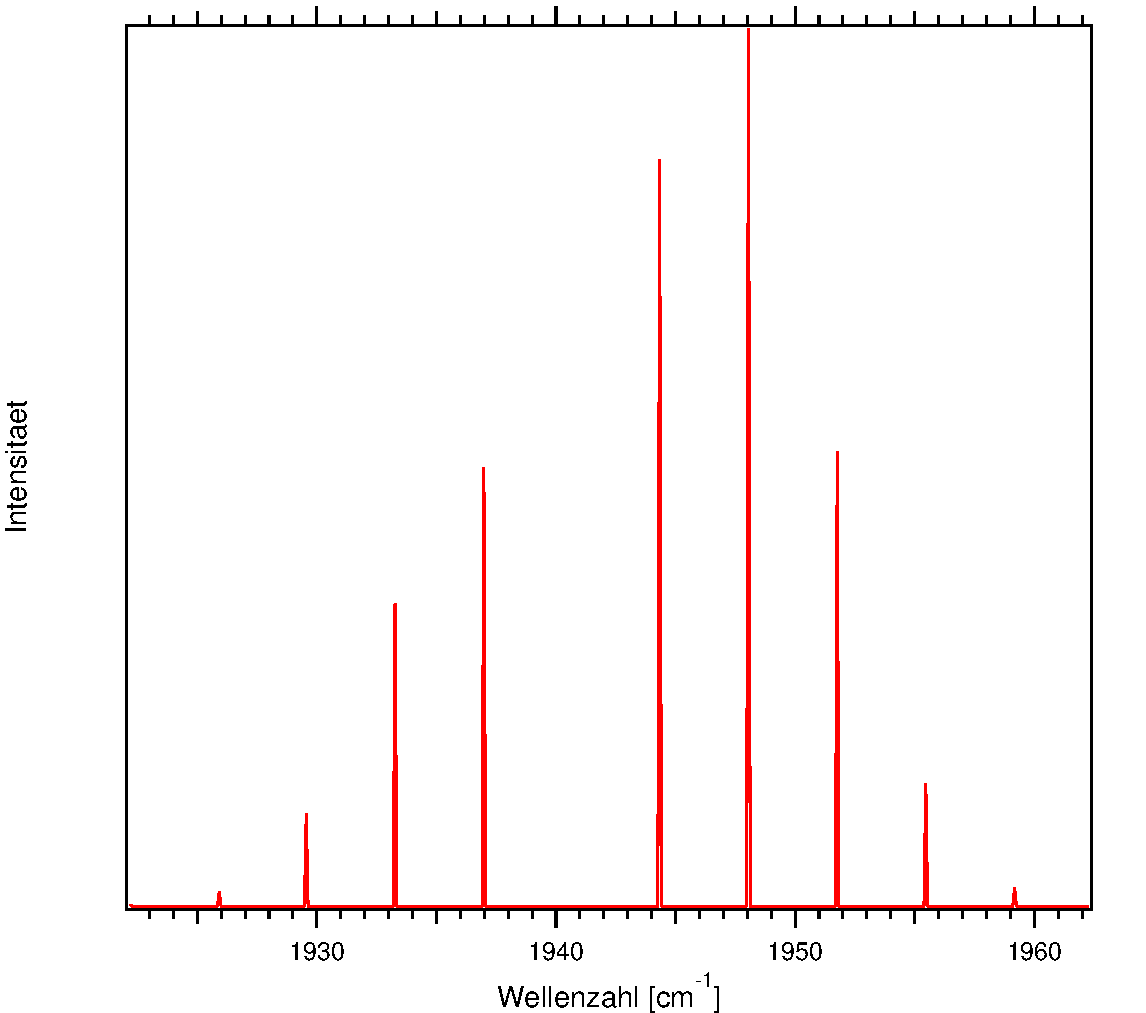
\includegraphics[width=\linewidth]{Bilder/10CO.pdf}
	\caption{berechnetes Rotationsschwingungsspektrum bei 10~K}
	\end{minipage}
\begin{minipage}{0.47\linewidth}
	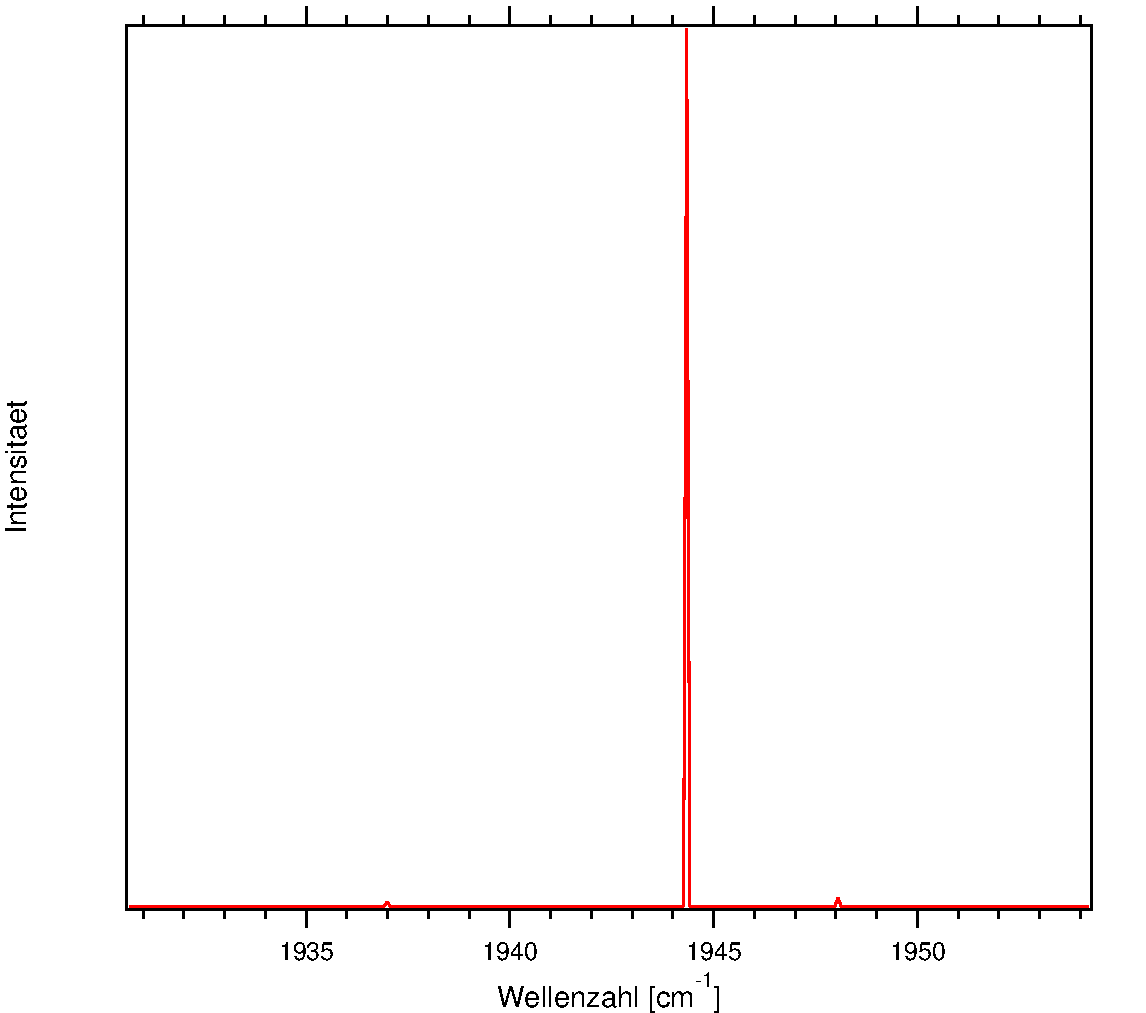
\includegraphics[width=\linewidth]{Bilder/1CO.pdf}
	\caption{berechnetes Rotationsschwingungsspektrum bei 1~K}
	\end{minipage}
	
	\caption{CO 10 und 1 Kelvin}
	
	
%	\label{•}
\end{figure}

\begin{figure}[H]
\centering	
	\begin{minipage}{0.47\linewidth}
	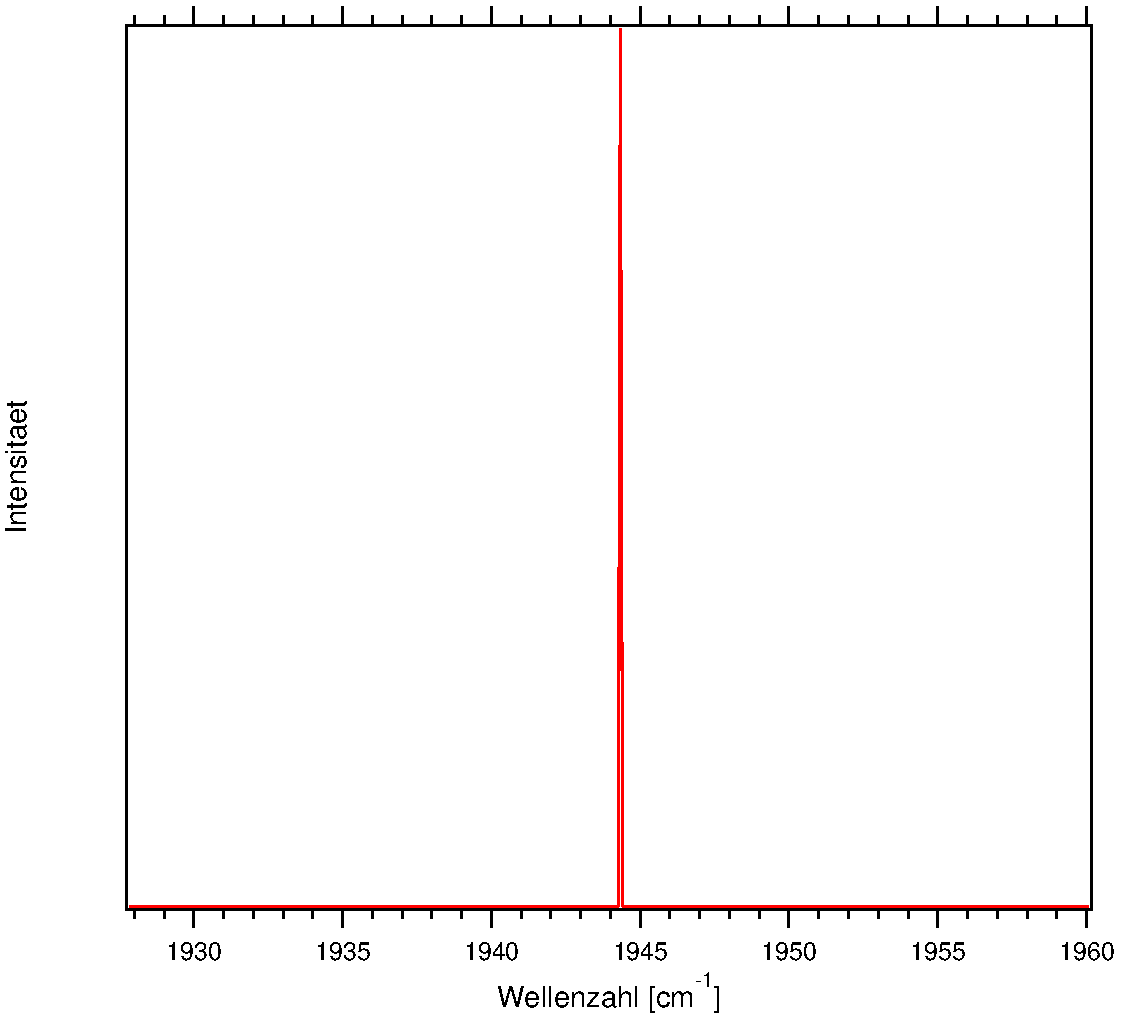
\includegraphics[width=\linewidth]{Bilder/001CO.pdf}
	\caption{berechnetes Rotationsschwingungsspektrum bei 10~K}
	\end{minipage}

	\caption{CO 10 und 1 Kelvin}
	
	
%	\label{}
\end{figure}


Bilden Sie daraus einen Satz Abbildungen und erklären Sie die Beobachtung! Wieviel Linien erhält man für T=0.01K? Zu welchem Zweig gehört sie? (-1 geht nicht daher +1)



\begin{figure}[H]
	
	\begin{minipage}{0.5\textwidth}
	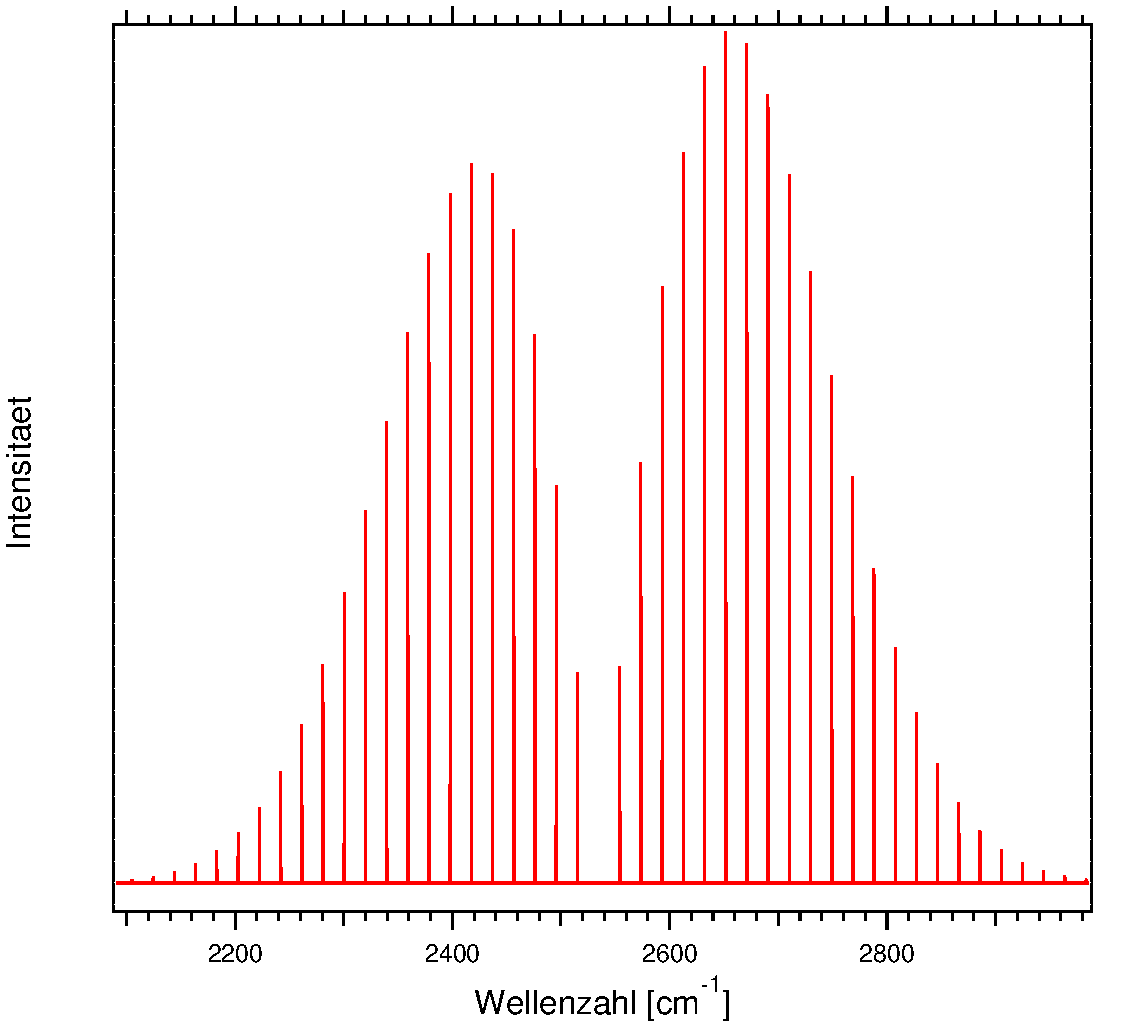
\includegraphics[width=\textwidth]{Bilder/1000HCL.pdf}
	\caption{berechnetes Rotationsschwingungsspektrum bei 1000 Kelvin}
	\end{minipage}
\begin{minipage}{0.5\textwidth}
	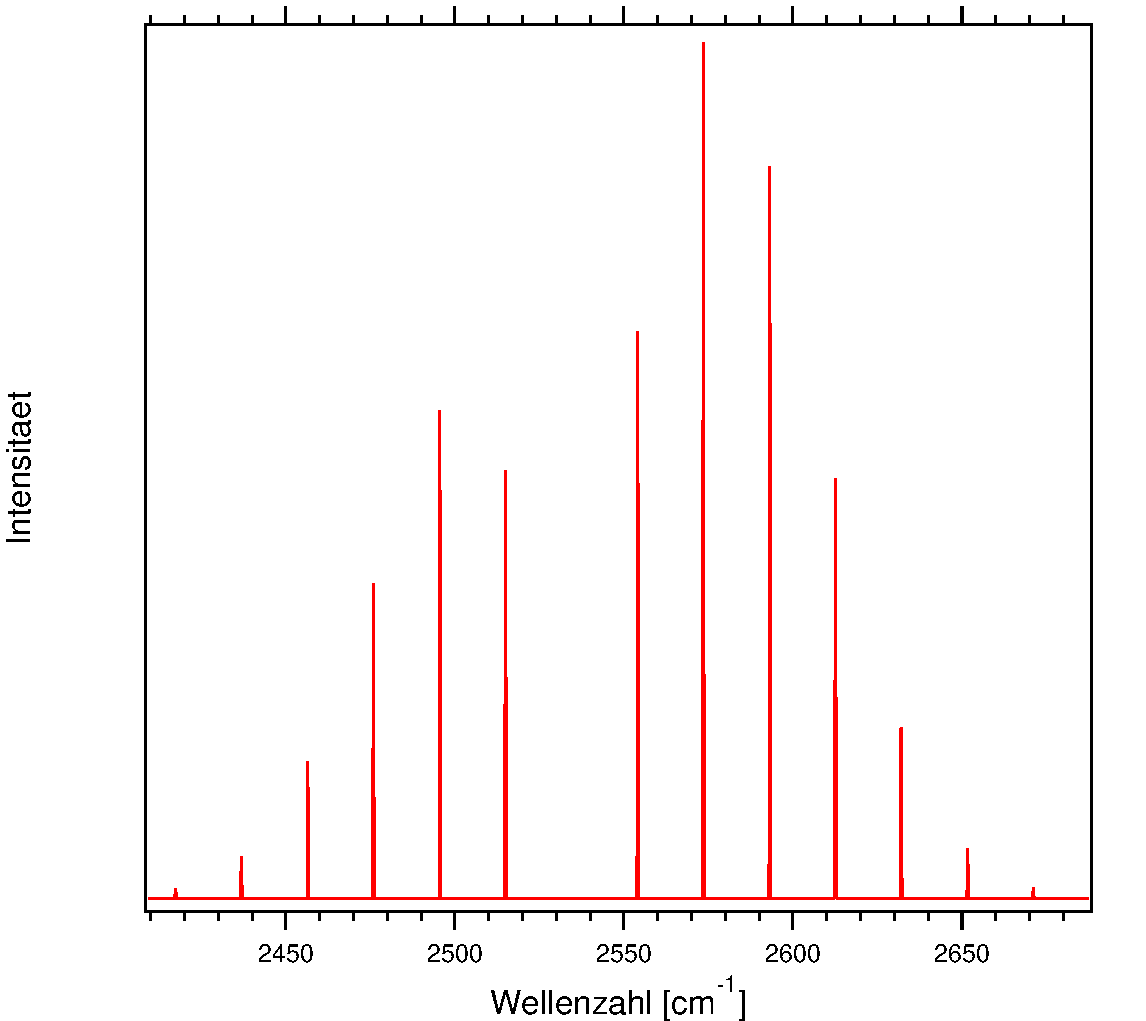
\includegraphics[width=\textwidth]{Bilder/100HCL.pdf}
	\caption{berechnetes Rotationsschwingungsspektrum bei 100 Kelvin}
	\end{minipage}	
	
	\caption{HCL 1000 und 100 Kelvin}
	
	
%	\label{1}
\end{figure}

\begin{figure}[H]
\centering	
	\begin{minipage}{0.47\linewidth}
	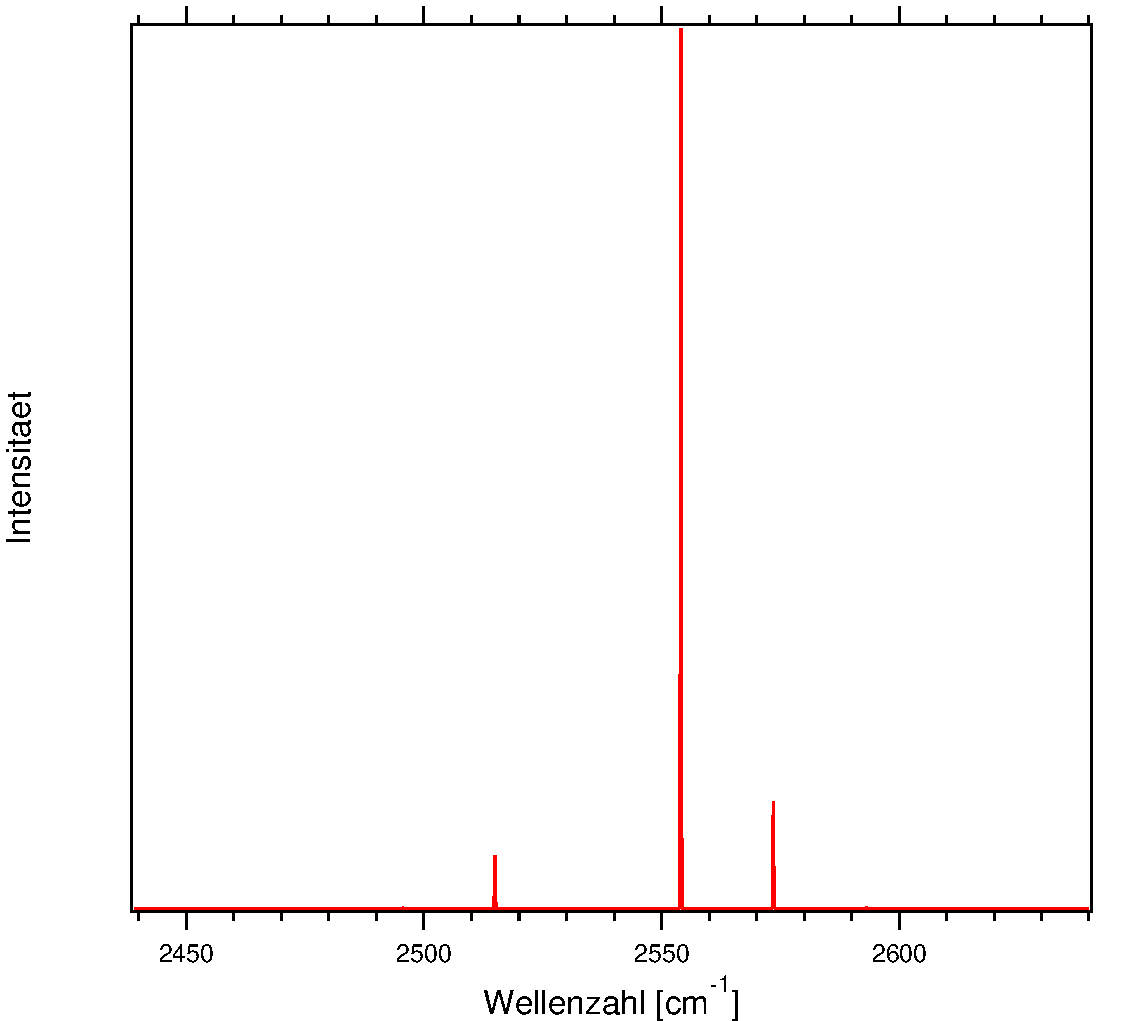
\includegraphics[width=\linewidth]{Bilder/10HCL.pdf}
	\caption{berechnetes Rotationsschwingungsspektrum bei 10~K}
	\end{minipage}
\begin{minipage}{0.47\linewidth}
	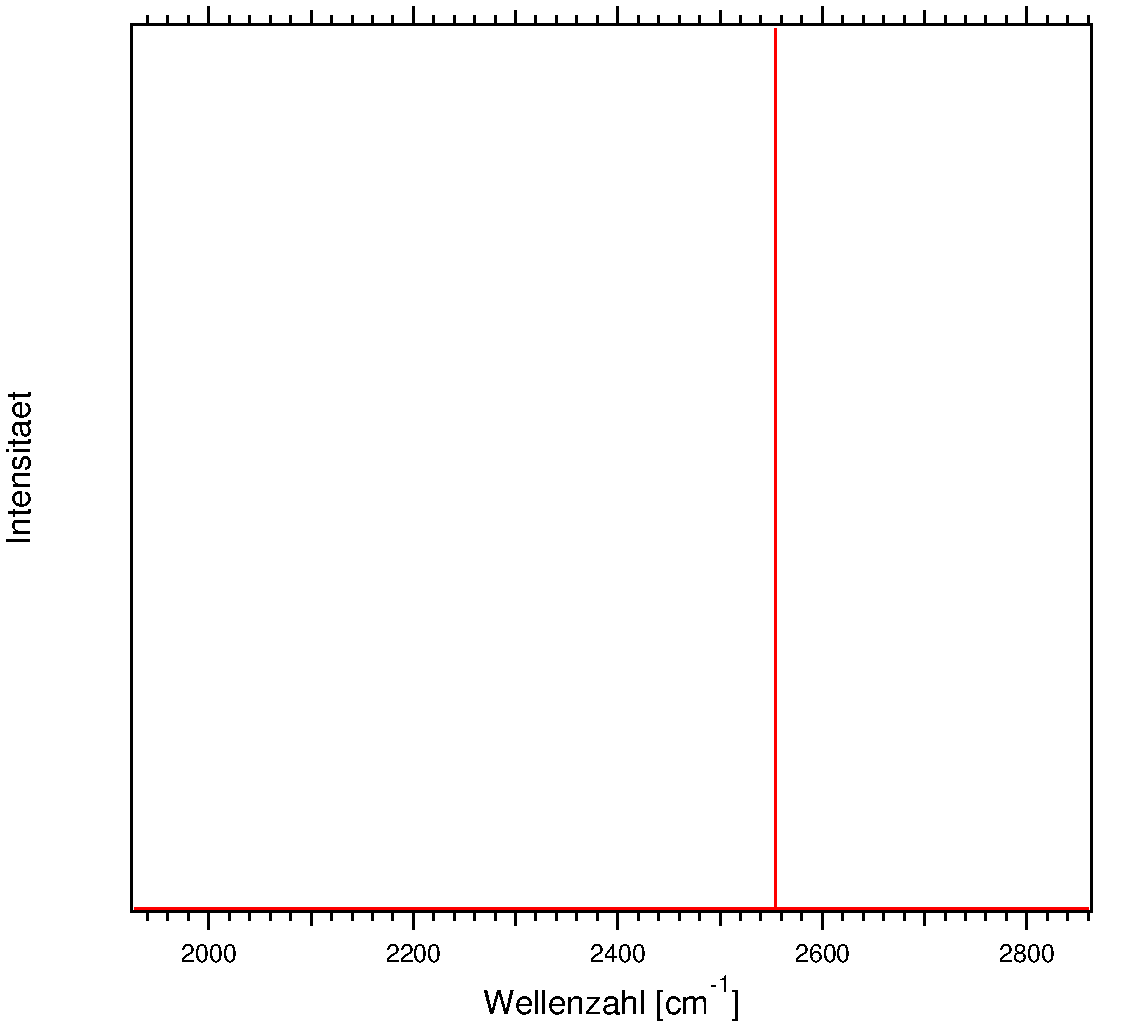
\includegraphics[width=\linewidth]{Bilder/1HCL.pdf}
	\caption{berechnetes Rotationsschwingungsspektrum bei 1~K}
	\end{minipage}
	
	\caption{HCL 10 und 1 Kelvin}
	
	
	
\end{figure}

\begin{figure}[H]
\centering	
	\begin{minipage}{0.47\linewidth}
	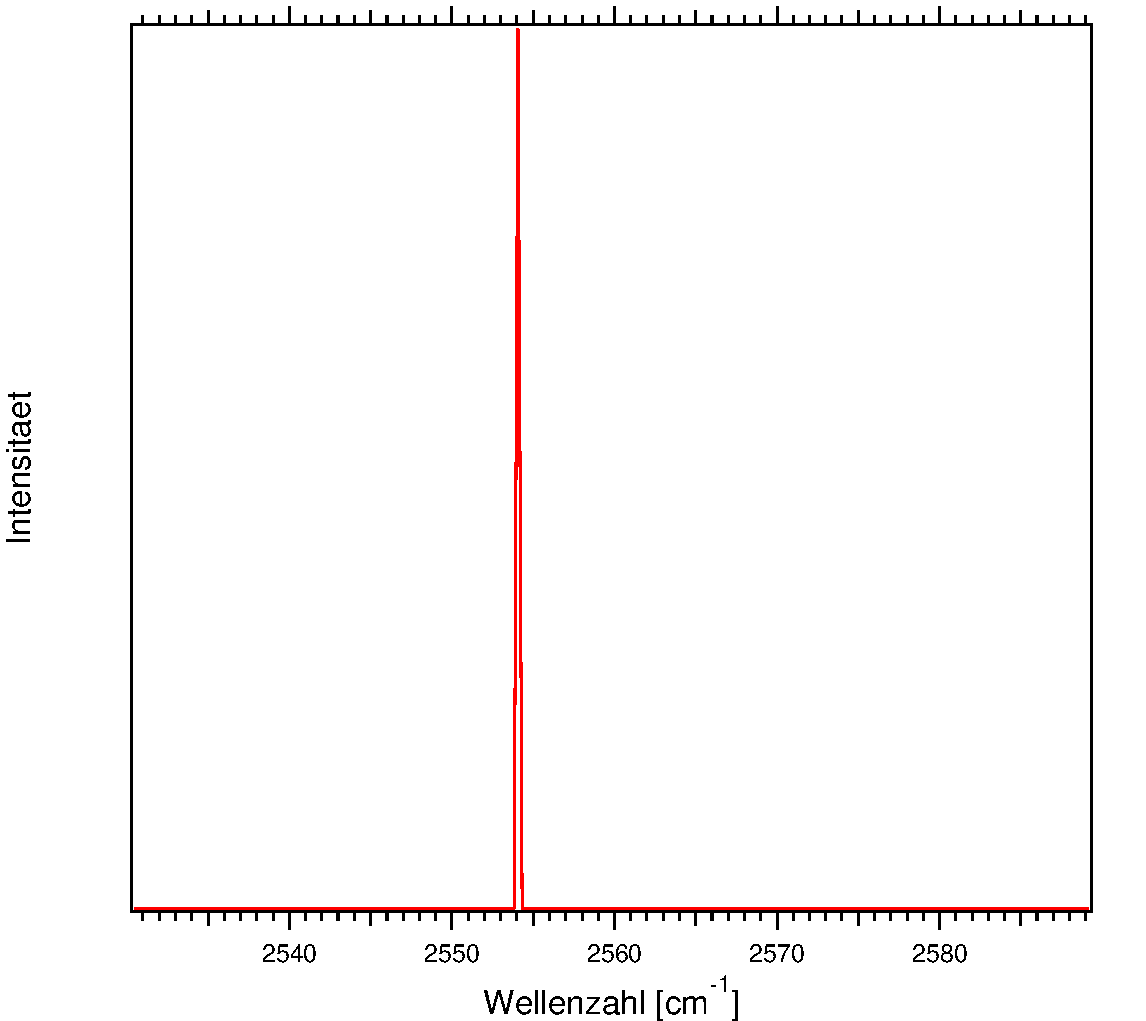
\includegraphics[width=\linewidth]{Bilder/001HCL.pdf}
	\caption{berechnetes Rotationsschwingungsspektrum bei 10~K}
	\end{minipage}

	\caption{HCL 10 und 1 Kelvin}
	
	
%	\label{3}
\end{figure}


\section{Rohdaten}

